{\color{red} Tarea de tv cable y su uso en acceso a internet:}



\begin{itemize}
\item {\color{red} Ancho de banda de TV cable.}\\
La televisión de aire tradicional se expandió a nivel mundial a lo largo de las décadas de 1940 y 1950, transmitiendo en las bandas VHF (Very High Frequency) entre los canales 2 a 13 (a lo largo de las frecuencias de 54 MHz a 216 MHz). Hacía una utilización parcial de esas bandas, que también estaban ocupadas por señales de radio (FM, marítima, aérea, de emergencias, radioaficionados, etcétera), distribuyendo los canales en distintas partes de ese espectro. A un canal de radiofrecuencia (RF) de televisión se le asignan 6 MHz\footnote{Las señales de TV transmiten señales de audio y video con una calidad decente. Por lo tanto, el ancho de banda requerido es mayor y está por debajo del rango de 6 MHZ.} de ancho de banda para la transmisión por aire en la banda de frecuencia VHF o UHF. En 1982, la Unión Internacional de Telecomunicaciones (UIT) estableció el uso primario para telecomunicaciones inalámbricas de la banda de 806 MHz a 890 MHz en América.

\begin{figure}[ht!]
\centering
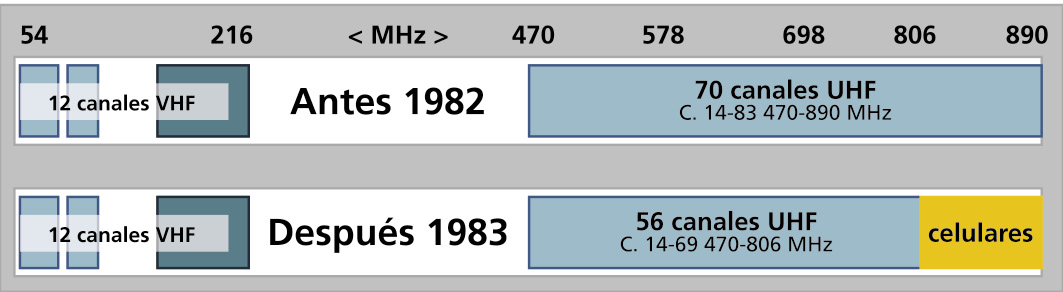
\includegraphics[scale=0.33]{Imagenes/fontanels-03_opt.jpeg}
\end{figure}

\item {\color{red} ¿Como se distribuyen los canales en este ancho de banda?}\\
En la actualidad, la televisión analógica en Bolivia sigue la distribución de canales sugerida para la Región 2 de la   UIT-R, donde las bandas de operación de los canales se distribuyen en el espectro de frecuencias VHF (30 a 300 MHz) y UHF (300 a 3000 MHz).

\begin{figure}[ht!]
\centering
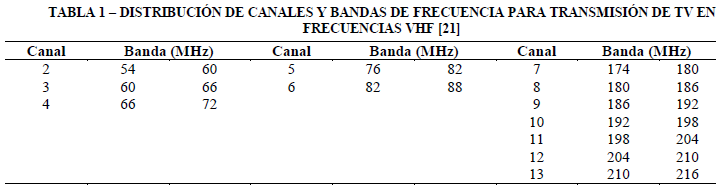
\includegraphics[scale=0.5]{Imagenes/a09_table_01.png}
\end{figure}

\begin{figure}[ht!]
\centering
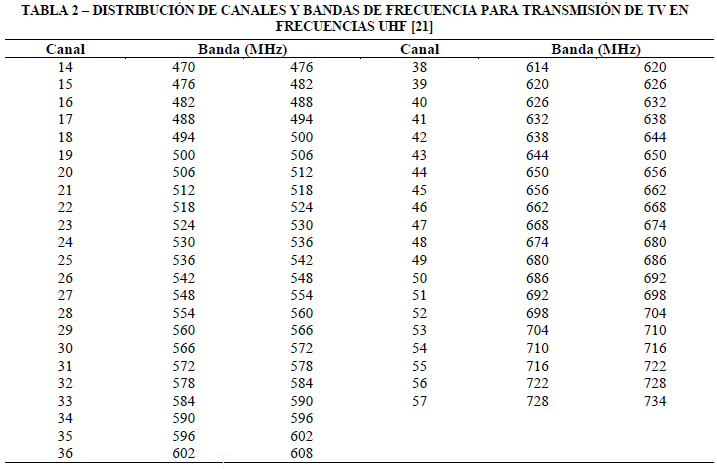
\includegraphics[scale=0.5]{Imagenes/a09_table_02.png}
\end{figure}
A través de la Ley de Telecomunicaciones del año 2011, Bolivia ha optado por un modelo en el que los radiocanales dedicados a la difusión de televisión analógica se distribuyen de manera porcentual en cada área de servicio definida por la ATT, de la siguiente manera:
\begin{itemize}
\item Estado: 33\%.
\item Comercial: 33\%.
\item Social comunitario: 17\%.
\item Pueblos de indígena originario campesinos, y comunidades interculturales y afrobolivianas: 17\%.
\end{itemize}

\item {\color{red} ¿Cuales son los utilizados para Tx datos?} \\
En el concepto de redes CATV multiservicios la banda de frecuencias se ha ampliado y reasignado como se indica a continuación:

\begin{figure}[ht!]
\centering
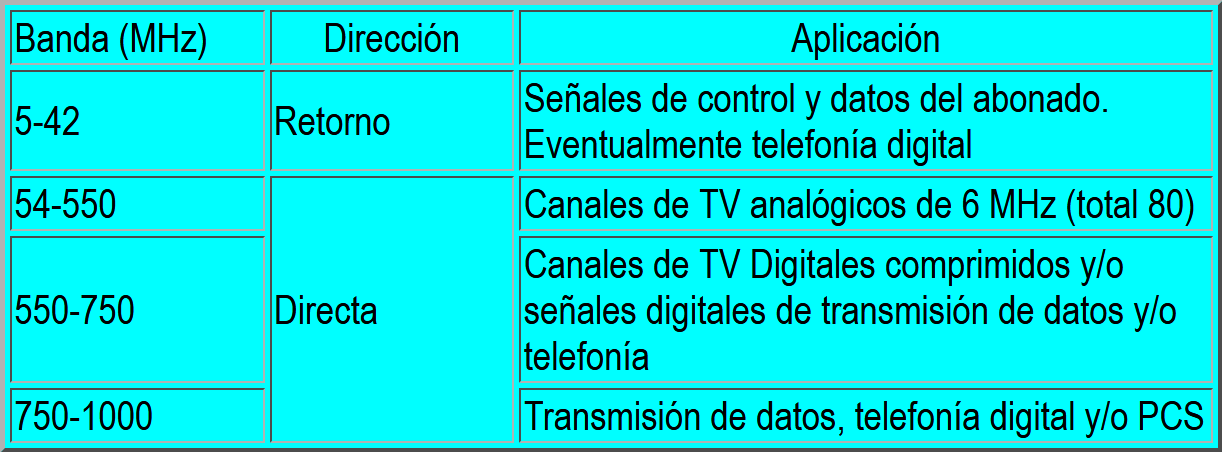
\includegraphics[scale=0.2]{Imagenes/tx.png}
\end{figure}


\item {\color{red} ¿Como funcionan los canales analogicos?}\\
La televisión analógica transmite la programación en una señal continua. Esta señal varía en amplitud, dependiendo de la información contenida en la imagen. Es una especie de transcripción de la música en discos de vinilo; la señal de televisión sube y baja dependiendo de lo que se está transmitiendo. \\
Esta señal analógica se transmite en una frecuencia de radio particular. A cada estación de televisión se le asigna una frecuencia particular que corresponde a su número de canal. Cuando sintoniza su televisor en un canal determinado, en realidad está eligiendo recibir transmisiones en esa frecuencia en particular. \\
Debido a su naturaleza, esta señal analógica está lejos de ser perfecta. Puede que no siempre reproduzca exactamente la programación original. Puede deteriorarse fácilmente a largas distancias. Y también puede sufrir interferencias de otras fuentes, produciendo imágenes fantasma, estática y "nieve".\\ Además, la televisión analógica es ineficaz. Cada canal de VHF o UHF ocupa una gran cantidad de ancho de banda valioso. La tecnología digital más eficiente puede colocar cuatro o más canales en un solo canal analógico. Y eso tiene muchos beneficios potenciales.
\item {\color{red} ¿Como funcionan los canales HD (digitales)? }\\
Una señal de TV digital, por otro lado, transmite en "paquetes" de datos comprimidos. Los datos utilizan una combinación de 1 y 0, similar a la computadora. Debido a que utiliza esta forma, las señales digitales no experimentan la misma interferencia o pérdida de señal que las señales de TV analógicas. Eso significa que se puede tener una imagen clara y constante, audio de alta calidad y sin estática ni "nieve". Una señal de TV digital también es una tecnología más eficiente. Una transmisión digital requiere menos ancho de banda en comparación con una señal analógica similar.
\end{itemize}

\begin{thebibliography}{9}
\bibitem{tutorialspoint} 
REVISIÓN Y ANÁLISIS CRÍTICO SOBRE LA IMPLEMENTACIÓN DE LA TELEVISIÓN DIGITAL TERRESTRE  EN BOLIVIA. Gustavo Siles \& Andrés Laguna, Laboratorio de Radiocomunicaciones,Laboratorio de Investigación en Comunicación y Humanidades, Universidad Privada Boliviana. \href{http://www.scielo.org.bo/scielo.php?pid=S2518-44312019000100009{\&}script=sci{\_}arttext}{http://www.scielo.org.bo/scielo.php?pid=S2518-44312019000100009{\&}script=sci{\_}arttext}, 26 junio 2019.

\bibitem{tutorialspoint2} 
Frequency Bands allocated to Terrestrial Broadcasting Services \href{https://www.itu.int/en/ITU-R/terrestrial/broadcast/Pages/Bands.aspx}{https://www.itu.int/en/ITU-R/terrestrial/broadcast/Pages/Bands.aspx}

\bibitem{tutorialspoint3} 
School of Computing. Dublin City University, Dr. Mark Humphrys. \href{https://www.computing.dcu.ie/~humphrys/Notes/Networks/physical.cable.html}{https://www.computing.dcu.ie/~humphrys/Notes/Networks/physical.cable.html}


\bibitem{tutorialspoint4} 
Analog Versus Digital TV: What's the Difference? \href{https://www.informit.com/articles/article.aspx?p=1245329}{https://www.informit.com/articles/article.aspx?p=1245329}

\bibitem{tutorialspoint4} 
Distribución de frecuencias de la TV Abierta y del CATV. \href{https://www.spw.cl/catv/catv0310.htm}{https://www.spw.cl/catv/catv0310.htm}

\end{thebibliography}

